% Created 2019-09-24 Tue 12:56
% Intended LaTeX compiler: pdflatex
\documentclass[11pt]{article}
\usepackage[utf8]{inputenc}
\usepackage[T1]{fontenc}
\usepackage{graphicx}
\usepackage{grffile}
\usepackage{longtable}
\usepackage{wrapfig}
\usepackage{rotating}
\usepackage[normalem]{ulem}
\usepackage{amsmath}
\usepackage{textcomp}
\usepackage{amssymb}
\usepackage{capt-of}
\usepackage{hyperref}
\usepackage[newfloat]{minted}
\usepackage{caption}
\author{Yi Zhang}
\date{\today}
\title{Two-compartment model solved using Torsten's \texttt{pmx\_solve\_twocpt} function}
\hypersetup{
 pdfauthor={Yi Zhang},
 pdftitle={Two-compartment model solved using Torsten's \texttt{pmx\_solve\_twocpt} function},
 pdfkeywords={},
 pdfsubject={},
 pdfcreator={Emacs 25.3.1 (Org mode 9.1.3)}, 
 pdflang={English}}
\begin{document}

\maketitle
\section{Model}
\label{sec:org58d8ed1}
We consider fitting a single-patient two-compartment model with linear absorption,
to demonstrate the usage of \texttt{pmx\_solve\_twocpt} function.
\section{Build}
\label{sec:orga0a39de}
\begin{minted}[breaklines=true,fontsize=\footnotesize,breakanywhere=true]{bash}
make ../example-models/twocpt_model/twocpt_model
\end{minted}
\section{Run}
\label{sec:orgd4c8ebf}
Using \texttt{cmdstan}
\begin{minted}[breaklines=true,fontsize=\footnotesize,breakanywhere=true]{bash}
for i in {1..4}; do ./TwoCptModel sample random seed=3892749 id=$i data file=TwoCptModel.data.R init=TwoCptModel.init.R output file=output_$i.csv; done
\end{minted}
\section{Results}
\label{sec:orgcaa9a49}
\texttt{./result/} directory contains Stan output from the above
run. To examine the results in \texttt{R}, we use \texttt{bayesplot} and \texttt{rstan}
\begin{minted}[breaklines=true,fontsize=\footnotesize,breakanywhere=true]{r}
library(bayesplot)
library(rstan)
fit <- read_stan_csv(list.files(path="result", pattern="*.csv", full.names=TRUE))
\end{minted}

\subsection{Scatter plot diagnostic}
\label{sec:org55e9152}
\begin{minted}[breaklines=true,fontsize=\footnotesize,breakanywhere=true]{r}
mcmc_scatter(as.matrix(fit), pars = c("CL", "ka"), np = nuts_params(fit),
             np_style = scatter_style_np(div_color = "green", div_alpha = 0.8))

\end{minted}

\begin{center}
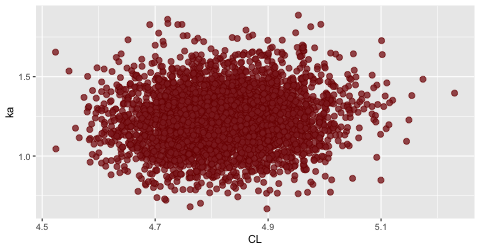
\includegraphics[width=.9\linewidth]{result/scatter.png}
\end{center}

\subsection{Energy  plot diagnostic}
\label{sec:org84300d8}
\begin{minted}[breaklines=true,fontsize=\footnotesize,breakanywhere=true]{r}
color_scheme_set("red");
np <- nuts_params(fit);
mcmc_nuts_energy(np) + ggtitle("NUTS Energy Diagnostic")
\end{minted}

\begin{center}
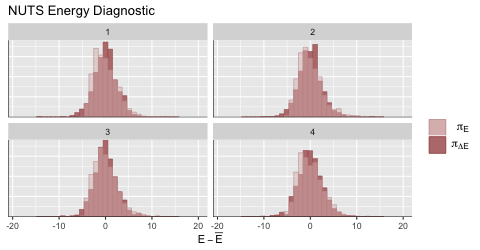
\includegraphics[width=.9\linewidth]{result/energy.png}
\end{center}
\end{document}
